% Created by tikzDevice version 0.12.3.1 on 2021-06-16 15:27:58
% !TEX encoding = UTF-8 Unicode
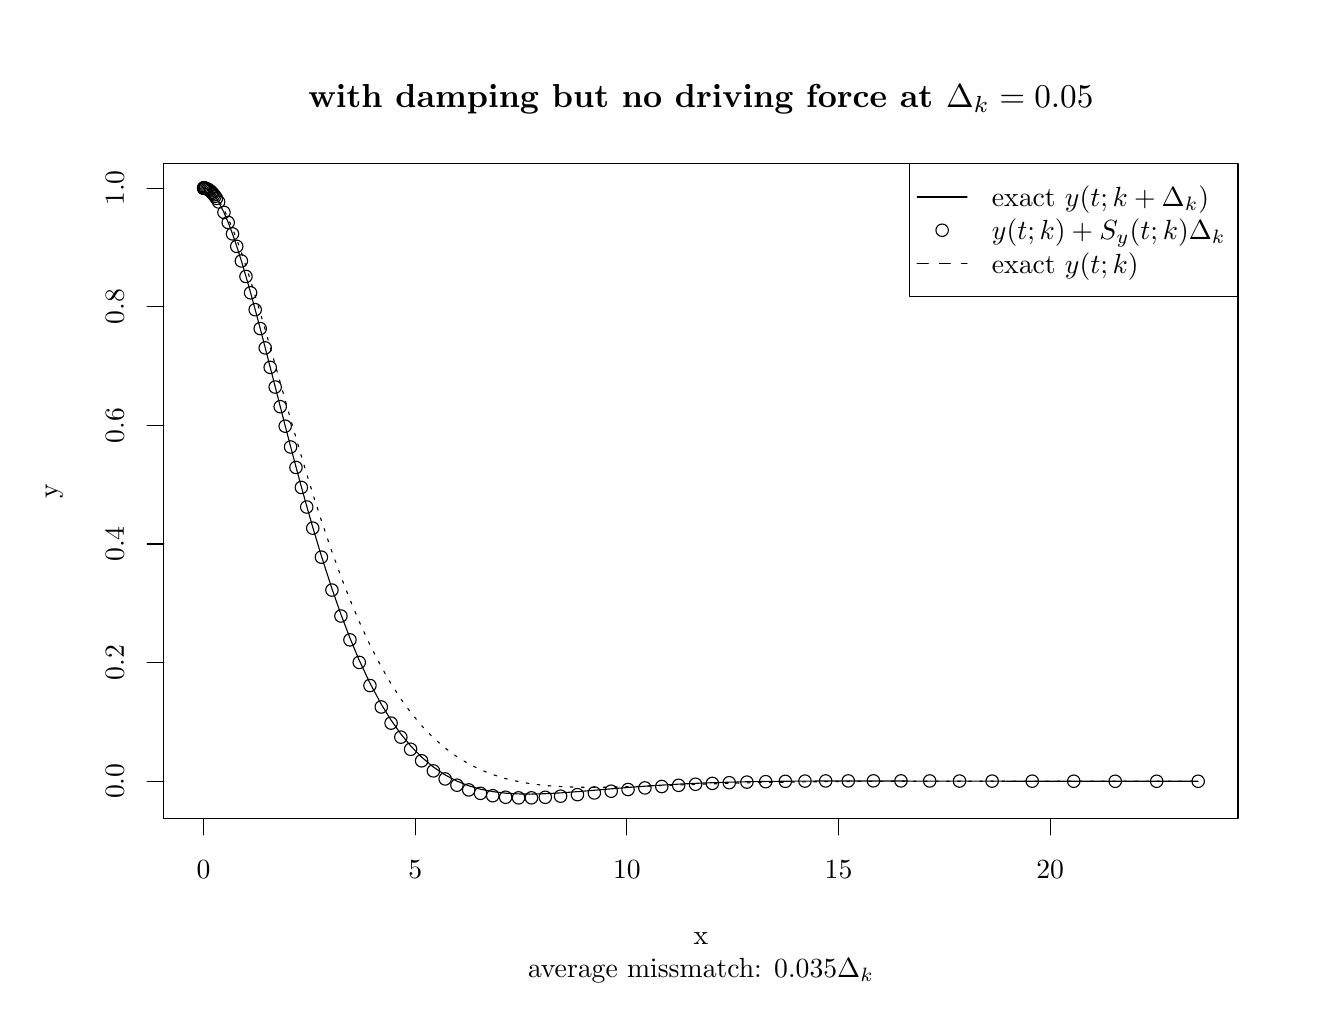
\begin{tikzpicture}[x=1pt,y=1pt]
\definecolor{fillColor}{RGB}{255,255,255}
\path[use as bounding box,fill=fillColor,fill opacity=0.00] (0,0) rectangle (462.53,346.90);
\begin{scope}
\path[clip] ( 49.20, 61.20) rectangle (437.33,297.70);
\definecolor{drawColor}{RGB}{0,0,0}

\path[draw=drawColor,line width= 0.4pt,line join=round,line cap=round] ( 63.58,288.94) --
	( 63.60,288.94) --
	( 63.63,288.94) --
	( 63.66,288.94) --
	( 63.70,288.93) --
	( 63.73,288.93) --
	( 63.76,288.93) --
	( 63.79,288.93) --
	( 63.84,288.92) --
	( 63.91,288.92) --
	( 64.04,288.90) --
	( 64.27,288.85) --
	( 64.77,288.67) --
	( 65.18,288.46) --
	( 65.60,288.18) --
	( 66.02,287.85) --
	( 66.44,287.46) --
	( 66.86,287.02) --
	( 67.28,286.52) --
	( 67.70,285.97) --
	( 68.22,285.21) --
	( 69.00,283.93) --
	( 70.92,280.16) --
	( 72.46,276.51) --
	( 74.01,272.40) --
	( 75.55,267.88) --
	( 77.22,262.61) --
	( 78.88,257.00) --
	( 80.55,251.12) --
	( 82.21,245.01) --
	( 84.02,238.20) --
	( 85.83,231.25) --
	( 87.63,224.21) --
	( 89.44,217.14) --
	( 91.25,210.07) --
	( 93.05,203.04) --
	( 95.00,195.55) --
	( 96.95,188.19) --
	( 98.89,180.99) --
	(100.84,173.97) --
	(103.01,166.38) --
	(106.14,155.97) --
	(109.94,144.18) --
	(113.19,134.89) --
	(116.45,126.35) --
	(119.81,118.31) --
	(123.68,110.06) --
	(127.77,102.41) --
	(131.31, 96.68) --
	(134.84, 91.69) --
	(138.37, 87.39) --
	(142.35, 83.30) --
	(146.61, 79.72) --
	(150.86, 76.87) --
	(155.11, 74.64) --
	(159.37, 72.96) --
	(163.62, 71.72) --
	(168.05, 70.85) --
	(172.71, 70.28) --
	(177.38, 70.01) --
	(182.04, 69.96) --
	(187.03, 70.09) --
	(192.57, 70.39) --
	(198.66, 70.84) --
	(204.76, 71.34) --
	(210.85, 71.85) --
	(216.94, 72.35) --
	(223.04, 72.80) --
	(229.13, 73.20) --
	(235.23, 73.55) --
	(241.32, 73.84) --
	(247.41, 74.07) --
	(253.51, 74.26) --
	(259.89, 74.41) --
	(266.67, 74.52) --
	(273.77, 74.60) --
	(280.87, 74.65) --
	(288.35, 74.68) --
	(296.52, 74.69) --
	(305.61, 74.69) --
	(315.56, 74.67) --
	(325.94, 74.65) --
	(336.72, 74.63) --
	(348.51, 74.62) --
	(363.00, 74.60) --
	(377.99, 74.59) --
	(392.98, 74.59) --
	(407.96, 74.59) --
	(422.95, 74.59);
\end{scope}
\begin{scope}
\path[clip] (  0.00,  0.00) rectangle (462.53,346.90);
\definecolor{drawColor}{RGB}{0,0,0}

\path[draw=drawColor,line width= 0.4pt,line join=round,line cap=round] ( 63.58, 61.20) -- (369.49, 61.20);

\path[draw=drawColor,line width= 0.4pt,line join=round,line cap=round] ( 63.58, 61.20) -- ( 63.58, 55.20);

\path[draw=drawColor,line width= 0.4pt,line join=round,line cap=round] (140.06, 61.20) -- (140.06, 55.20);

\path[draw=drawColor,line width= 0.4pt,line join=round,line cap=round] (216.54, 61.20) -- (216.54, 55.20);

\path[draw=drawColor,line width= 0.4pt,line join=round,line cap=round] (293.02, 61.20) -- (293.02, 55.20);

\path[draw=drawColor,line width= 0.4pt,line join=round,line cap=round] (369.49, 61.20) -- (369.49, 55.20);

\node[text=drawColor,anchor=base,inner sep=0pt, outer sep=0pt, scale=  1.00] at ( 63.58, 39.60) {0};

\node[text=drawColor,anchor=base,inner sep=0pt, outer sep=0pt, scale=  1.00] at (140.06, 39.60) {5};

\node[text=drawColor,anchor=base,inner sep=0pt, outer sep=0pt, scale=  1.00] at (216.54, 39.60) {10};

\node[text=drawColor,anchor=base,inner sep=0pt, outer sep=0pt, scale=  1.00] at (293.02, 39.60) {15};

\node[text=drawColor,anchor=base,inner sep=0pt, outer sep=0pt, scale=  1.00] at (369.49, 39.60) {20};

\path[draw=drawColor,line width= 0.4pt,line join=round,line cap=round] ( 49.20, 74.59) -- ( 49.20,288.94);

\path[draw=drawColor,line width= 0.4pt,line join=round,line cap=round] ( 49.20, 74.59) -- ( 43.20, 74.59);

\path[draw=drawColor,line width= 0.4pt,line join=round,line cap=round] ( 49.20,117.46) -- ( 43.20,117.46);

\path[draw=drawColor,line width= 0.4pt,line join=round,line cap=round] ( 49.20,160.33) -- ( 43.20,160.33);

\path[draw=drawColor,line width= 0.4pt,line join=round,line cap=round] ( 49.20,203.20) -- ( 43.20,203.20);

\path[draw=drawColor,line width= 0.4pt,line join=round,line cap=round] ( 49.20,246.07) -- ( 43.20,246.07);

\path[draw=drawColor,line width= 0.4pt,line join=round,line cap=round] ( 49.20,288.94) -- ( 43.20,288.94);

\node[text=drawColor,rotate= 90.00,anchor=base,inner sep=0pt, outer sep=0pt, scale=  1.00] at ( 34.80, 74.59) {0.0};

\node[text=drawColor,rotate= 90.00,anchor=base,inner sep=0pt, outer sep=0pt, scale=  1.00] at ( 34.80,117.46) {0.2};

\node[text=drawColor,rotate= 90.00,anchor=base,inner sep=0pt, outer sep=0pt, scale=  1.00] at ( 34.80,160.33) {0.4};

\node[text=drawColor,rotate= 90.00,anchor=base,inner sep=0pt, outer sep=0pt, scale=  1.00] at ( 34.80,203.20) {0.6};

\node[text=drawColor,rotate= 90.00,anchor=base,inner sep=0pt, outer sep=0pt, scale=  1.00] at ( 34.80,246.07) {0.8};

\node[text=drawColor,rotate= 90.00,anchor=base,inner sep=0pt, outer sep=0pt, scale=  1.00] at ( 34.80,288.94) {1.0};

\path[draw=drawColor,line width= 0.4pt,line join=round,line cap=round] ( 49.20, 61.20) --
	(437.33, 61.20) --
	(437.33,297.70) --
	( 49.20,297.70) --
	( 49.20, 61.20);
\end{scope}
\begin{scope}
\path[clip] (  0.00,  0.00) rectangle (462.53,346.90);
\definecolor{drawColor}{RGB}{0,0,0}

\node[text=drawColor,anchor=base,inner sep=0pt, outer sep=0pt, scale=  1.20] at (243.26,318.16) {\bfseries  with damping but no driving force at $\Delta_k = 0.05$};

\node[text=drawColor,anchor=base,inner sep=0pt, outer sep=0pt, scale=  1.00] at (243.26,  3.60) {average missmatch: $0.035 \Delta_k$};

\node[text=drawColor,anchor=base,inner sep=0pt, outer sep=0pt, scale=  1.00] at (243.26, 15.60) {x};

\node[text=drawColor,rotate= 90.00,anchor=base,inner sep=0pt, outer sep=0pt, scale=  1.00] at ( 10.80,179.45) {y};
\end{scope}
\begin{scope}
\path[clip] ( 49.20, 61.20) rectangle (437.33,297.70);
\definecolor{drawColor}{RGB}{0,0,0}

\path[draw=drawColor,line width= 0.4pt,line join=round,line cap=round] ( 63.58,288.94) circle (  2.25);

\path[draw=drawColor,line width= 0.4pt,line join=round,line cap=round] ( 63.60,288.94) circle (  2.25);

\path[draw=drawColor,line width= 0.4pt,line join=round,line cap=round] ( 63.63,288.94) circle (  2.25);

\path[draw=drawColor,line width= 0.4pt,line join=round,line cap=round] ( 63.66,288.93) circle (  2.25);

\path[draw=drawColor,line width= 0.4pt,line join=round,line cap=round] ( 63.70,288.93) circle (  2.25);

\path[draw=drawColor,line width= 0.4pt,line join=round,line cap=round] ( 63.73,288.93) circle (  2.25);

\path[draw=drawColor,line width= 0.4pt,line join=round,line cap=round] ( 63.76,288.93) circle (  2.25);

\path[draw=drawColor,line width= 0.4pt,line join=round,line cap=round] ( 63.79,288.93) circle (  2.25);

\path[draw=drawColor,line width= 0.4pt,line join=round,line cap=round] ( 63.84,288.92) circle (  2.25);

\path[draw=drawColor,line width= 0.4pt,line join=round,line cap=round] ( 63.91,288.91) circle (  2.25);

\path[draw=drawColor,line width= 0.4pt,line join=round,line cap=round] ( 64.04,288.90) circle (  2.25);

\path[draw=drawColor,line width= 0.4pt,line join=round,line cap=round] ( 64.27,288.85) circle (  2.25);

\path[draw=drawColor,line width= 0.4pt,line join=round,line cap=round] ( 64.77,288.67) circle (  2.25);

\path[draw=drawColor,line width= 0.4pt,line join=round,line cap=round] ( 65.18,288.46) circle (  2.25);

\path[draw=drawColor,line width= 0.4pt,line join=round,line cap=round] ( 65.60,288.18) circle (  2.25);

\path[draw=drawColor,line width= 0.4pt,line join=round,line cap=round] ( 66.02,287.85) circle (  2.25);

\path[draw=drawColor,line width= 0.4pt,line join=round,line cap=round] ( 66.44,287.46) circle (  2.25);

\path[draw=drawColor,line width= 0.4pt,line join=round,line cap=round] ( 66.86,287.02) circle (  2.25);

\path[draw=drawColor,line width= 0.4pt,line join=round,line cap=round] ( 67.28,286.52) circle (  2.25);

\path[draw=drawColor,line width= 0.4pt,line join=round,line cap=round] ( 67.70,285.97) circle (  2.25);

\path[draw=drawColor,line width= 0.4pt,line join=round,line cap=round] ( 68.22,285.22) circle (  2.25);

\path[draw=drawColor,line width= 0.4pt,line join=round,line cap=round] ( 69.00,283.93) circle (  2.25);

\path[draw=drawColor,line width= 0.4pt,line join=round,line cap=round] ( 70.92,280.16) circle (  2.25);

\path[draw=drawColor,line width= 0.4pt,line join=round,line cap=round] ( 72.46,276.51) circle (  2.25);

\path[draw=drawColor,line width= 0.4pt,line join=round,line cap=round] ( 74.01,272.39) circle (  2.25);

\path[draw=drawColor,line width= 0.4pt,line join=round,line cap=round] ( 75.55,267.87) circle (  2.25);

\path[draw=drawColor,line width= 0.4pt,line join=round,line cap=round] ( 77.22,262.60) circle (  2.25);

\path[draw=drawColor,line width= 0.4pt,line join=round,line cap=round] ( 78.88,256.99) circle (  2.25);

\path[draw=drawColor,line width= 0.4pt,line join=round,line cap=round] ( 80.55,251.09) circle (  2.25);

\path[draw=drawColor,line width= 0.4pt,line join=round,line cap=round] ( 82.21,244.98) circle (  2.25);

\path[draw=drawColor,line width= 0.4pt,line join=round,line cap=round] ( 84.02,238.16) circle (  2.25);

\path[draw=drawColor,line width= 0.4pt,line join=round,line cap=round] ( 85.83,231.19) circle (  2.25);

\path[draw=drawColor,line width= 0.4pt,line join=round,line cap=round] ( 87.63,224.14) circle (  2.25);

\path[draw=drawColor,line width= 0.4pt,line join=round,line cap=round] ( 89.44,217.04) circle (  2.25);

\path[draw=drawColor,line width= 0.4pt,line join=round,line cap=round] ( 91.25,209.95) circle (  2.25);

\path[draw=drawColor,line width= 0.4pt,line join=round,line cap=round] ( 93.05,202.90) circle (  2.25);

\path[draw=drawColor,line width= 0.4pt,line join=round,line cap=round] ( 95.00,195.38) circle (  2.25);

\path[draw=drawColor,line width= 0.4pt,line join=round,line cap=round] ( 96.95,187.98) circle (  2.25);

\path[draw=drawColor,line width= 0.4pt,line join=round,line cap=round] ( 98.89,180.75) circle (  2.25);

\path[draw=drawColor,line width= 0.4pt,line join=round,line cap=round] (100.84,173.69) circle (  2.25);

\path[draw=drawColor,line width= 0.4pt,line join=round,line cap=round] (103.01,166.05) circle (  2.25);

\path[draw=drawColor,line width= 0.4pt,line join=round,line cap=round] (106.14,155.57) circle (  2.25);

\path[draw=drawColor,line width= 0.4pt,line join=round,line cap=round] (109.94,143.68) circle (  2.25);

\path[draw=drawColor,line width= 0.4pt,line join=round,line cap=round] (113.19,134.30) circle (  2.25);

\path[draw=drawColor,line width= 0.4pt,line join=round,line cap=round] (116.45,125.68) circle (  2.25);

\path[draw=drawColor,line width= 0.4pt,line join=round,line cap=round] (119.81,117.54) circle (  2.25);

\path[draw=drawColor,line width= 0.4pt,line join=round,line cap=round] (123.68,109.19) circle (  2.25);

\path[draw=drawColor,line width= 0.4pt,line join=round,line cap=round] (127.77,101.43) circle (  2.25);

\path[draw=drawColor,line width= 0.4pt,line join=round,line cap=round] (131.31, 95.60) circle (  2.25);

\path[draw=drawColor,line width= 0.4pt,line join=round,line cap=round] (134.84, 90.53) circle (  2.25);

\path[draw=drawColor,line width= 0.4pt,line join=round,line cap=round] (138.37, 86.15) circle (  2.25);

\path[draw=drawColor,line width= 0.4pt,line join=round,line cap=round] (142.35, 81.98) circle (  2.25);

\path[draw=drawColor,line width= 0.4pt,line join=round,line cap=round] (146.61, 78.34) circle (  2.25);

\path[draw=drawColor,line width= 0.4pt,line join=round,line cap=round] (150.86, 75.43) circle (  2.25);

\path[draw=drawColor,line width= 0.4pt,line join=round,line cap=round] (155.11, 73.17) circle (  2.25);

\path[draw=drawColor,line width= 0.4pt,line join=round,line cap=round] (159.37, 71.46) circle (  2.25);

\path[draw=drawColor,line width= 0.4pt,line join=round,line cap=round] (163.62, 70.23) circle (  2.25);

\path[draw=drawColor,line width= 0.4pt,line join=round,line cap=round] (168.05, 69.36) circle (  2.25);

\path[draw=drawColor,line width= 0.4pt,line join=round,line cap=round] (172.71, 68.82) circle (  2.25);

\path[draw=drawColor,line width= 0.4pt,line join=round,line cap=round] (177.38, 68.59) circle (  2.25);

\path[draw=drawColor,line width= 0.4pt,line join=round,line cap=round] (182.04, 68.60) circle (  2.25);

\path[draw=drawColor,line width= 0.4pt,line join=round,line cap=round] (187.03, 68.80) circle (  2.25);

\path[draw=drawColor,line width= 0.4pt,line join=round,line cap=round] (192.57, 69.20) circle (  2.25);

\path[draw=drawColor,line width= 0.4pt,line join=round,line cap=round] (198.66, 69.75) circle (  2.25);

\path[draw=drawColor,line width= 0.4pt,line join=round,line cap=round] (204.76, 70.37) circle (  2.25);

\path[draw=drawColor,line width= 0.4pt,line join=round,line cap=round] (210.85, 71.00) circle (  2.25);

\path[draw=drawColor,line width= 0.4pt,line join=round,line cap=round] (216.94, 71.61) circle (  2.25);

\path[draw=drawColor,line width= 0.4pt,line join=round,line cap=round] (223.04, 72.18) circle (  2.25);

\path[draw=drawColor,line width= 0.4pt,line join=round,line cap=round] (229.13, 72.69) circle (  2.25);

\path[draw=drawColor,line width= 0.4pt,line join=round,line cap=round] (235.23, 73.13) circle (  2.25);

\path[draw=drawColor,line width= 0.4pt,line join=round,line cap=round] (241.32, 73.51) circle (  2.25);

\path[draw=drawColor,line width= 0.4pt,line join=round,line cap=round] (247.41, 73.82) circle (  2.25);

\path[draw=drawColor,line width= 0.4pt,line join=round,line cap=round] (253.51, 74.07) circle (  2.25);

\path[draw=drawColor,line width= 0.4pt,line join=round,line cap=round] (259.89, 74.28) circle (  2.25);

\path[draw=drawColor,line width= 0.4pt,line join=round,line cap=round] (266.67, 74.44) circle (  2.25);

\path[draw=drawColor,line width= 0.4pt,line join=round,line cap=round] (273.77, 74.57) circle (  2.25);

\path[draw=drawColor,line width= 0.4pt,line join=round,line cap=round] (280.87, 74.65) circle (  2.25);

\path[draw=drawColor,line width= 0.4pt,line join=round,line cap=round] (288.35, 74.70) circle (  2.25);

\path[draw=drawColor,line width= 0.4pt,line join=round,line cap=round] (296.52, 74.72) circle (  2.25);

\path[draw=drawColor,line width= 0.4pt,line join=round,line cap=round] (305.61, 74.73) circle (  2.25);

\path[draw=drawColor,line width= 0.4pt,line join=round,line cap=round] (315.56, 74.72) circle (  2.25);

\path[draw=drawColor,line width= 0.4pt,line join=round,line cap=round] (325.94, 74.70) circle (  2.25);

\path[draw=drawColor,line width= 0.4pt,line join=round,line cap=round] (336.72, 74.67) circle (  2.25);

\path[draw=drawColor,line width= 0.4pt,line join=round,line cap=round] (348.51, 74.65) circle (  2.25);

\path[draw=drawColor,line width= 0.4pt,line join=round,line cap=round] (363.00, 74.62) circle (  2.25);

\path[draw=drawColor,line width= 0.4pt,line join=round,line cap=round] (377.99, 74.60) circle (  2.25);

\path[draw=drawColor,line width= 0.4pt,line join=round,line cap=round] (392.98, 74.59) circle (  2.25);

\path[draw=drawColor,line width= 0.4pt,line join=round,line cap=round] (407.96, 74.59) circle (  2.25);

\path[draw=drawColor,line width= 0.4pt,line join=round,line cap=round] (422.95, 74.59) circle (  2.25);

\path[draw=drawColor,line width= 0.4pt,dash pattern=on 1pt off 3pt ,line join=round,line cap=round] ( 63.58,288.94) --
	( 63.60,288.94) --
	( 63.63,288.94) --
	( 63.66,288.94) --
	( 63.70,288.93) --
	( 63.73,288.93) --
	( 63.76,288.93) --
	( 63.79,288.93) --
	( 63.84,288.93) --
	( 63.91,288.92) --
	( 64.04,288.90) --
	( 64.27,288.86) --
	( 64.77,288.70) --
	( 65.18,288.52) --
	( 65.60,288.27) --
	( 66.02,287.98) --
	( 66.44,287.64) --
	( 66.86,287.25) --
	( 67.28,286.81) --
	( 67.70,286.32) --
	( 68.22,285.66) --
	( 69.00,284.53) --
	( 70.92,281.20) --
	( 72.46,277.98) --
	( 74.01,274.35) --
	( 75.55,270.35) --
	( 77.22,265.69) --
	( 78.88,260.71) --
	( 80.55,255.49) --
	( 82.21,250.05) --
	( 84.02,243.97) --
	( 85.83,237.75) --
	( 87.63,231.43) --
	( 89.44,225.06) --
	( 91.25,218.67) --
	( 93.05,212.29) --
	( 95.00,205.47) --
	( 96.95,198.73) --
	( 98.89,192.10) --
	(100.84,185.61) --
	(103.01,178.54) --
	(106.14,168.77) --
	(109.94,157.56) --
	(113.19,148.60) --
	(116.45,140.25) --
	(119.81,132.26) --
	(123.68,123.90) --
	(127.77,115.95) --
	(131.31,109.83) --
	(134.84,104.36) --
	(138.37, 99.50) --
	(142.35, 94.69) --
	(146.61, 90.29) --
	(150.86, 86.57) --
	(155.11, 83.45) --
	(159.37, 80.87) --
	(163.62, 78.76) --
	(168.05, 77.00) --
	(172.71, 75.55) --
	(177.38, 74.46) --
	(182.04, 73.65) --
	(187.03, 73.06) --
	(192.57, 72.65) --
	(198.66, 72.43) --
	(204.76, 72.38) --
	(210.85, 72.46) --
	(216.94, 72.61) --
	(223.04, 72.81) --
	(229.13, 73.03) --
	(235.23, 73.25) --
	(241.32, 73.46) --
	(247.41, 73.66) --
	(253.51, 73.84) --
	(259.89, 74.00) --
	(266.67, 74.14) --
	(273.77, 74.27) --
	(280.87, 74.37) --
	(288.35, 74.44) --
	(296.52, 74.51) --
	(305.61, 74.56) --
	(315.56, 74.59) --
	(325.94, 74.60) --
	(336.72, 74.61) --
	(348.51, 74.61) --
	(363.00, 74.61) --
	(377.99, 74.60) --
	(392.98, 74.60) --
	(407.96, 74.59) --
	(422.95, 74.59);
\definecolor{fillColor}{RGB}{255,255,255}

\path[draw=drawColor,line width= 0.4pt,line join=round,line cap=round,fill=fillColor] (318.74,297.70) rectangle (437.33,249.70);

\path[draw=drawColor,line width= 0.4pt,line join=round,line cap=round] (321.44,285.70) -- (339.44,285.70);

\path[draw=drawColor,line width= 0.4pt,dash pattern=on 4pt off 4pt ,line join=round,line cap=round] (321.44,261.70) -- (339.44,261.70);

\path[draw=drawColor,line width= 0.4pt,line join=round,line cap=round] (330.44,273.70) circle (  2.25);

\node[text=drawColor,anchor=base west,inner sep=0pt, outer sep=0pt, scale=  1.00] at (348.44,282.25) {exact $y(t;k+\Delta_k)$};

\node[text=drawColor,anchor=base west,inner sep=0pt, outer sep=0pt, scale=  1.00] at (348.44,270.25) {$y(t;k) + S_y(t;k) \Delta_k$};

\node[text=drawColor,anchor=base west,inner sep=0pt, outer sep=0pt, scale=  1.00] at (348.44,258.25) {exact $y(t;k)$};
\end{scope}
\end{tikzpicture}
